\documentclass[tikz]{standalone}

\usepackage{fontspec}

\usetikzlibrary{arrows}
\usetikzlibrary{calc}
\usetikzlibrary{decorations.pathreplacing}
\usetikzlibrary{positioning}
\usetikzlibrary{matrix}

\usepackage{fontspec}

\begin{document}

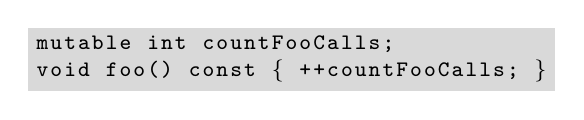
\begin{tikzpicture}
  [node distance=5mm, >=stealth',
  every node/.style={font=\footnotesize},
  every matrix/.style={fill=black!15, inner sep=1mm, row sep=0.5mm,
                        matrix of nodes, nodes in empty cells,
                        minimum height=0.5em, minimum width=.5em,
                        nodes={anchor=base, inner sep=0, font=\ttfamily\footnotesize}}]

  \matrix {
m & u & t & a & b & l & e &   & i & n & t &   & c & o & u & n & t & F & o & o & C & a & l & l & s & ; &   &   &   &   &   &   &   &   &   &   &   \\
v & o & i & d &   & f & o & o & ( & ) &   & c & o & n & s & t &   & \{ &   & + & + & c & o & u & n & t & F & o & o & C & a & l & l & s & ; &   & \} \\
  };
\end{tikzpicture}

\end{document}
